%!TEX root = ../../main.tex

\chapter{Grundlagen}\label{ch:grundlagen}
Dieses Kapitel befasst sich mit einigen Grundlagen, die zum Verständnis dieser Arbeit vonnöten sind. Die zwei nachfolgenden Unterkapitel können von derjenigen Leserschaft, die bereits Erfahrungen mit \textit{FNT Command} und vor allem dem \ac{CIF} hat, übersprungen werden.

\section{FNT Command}\label{sec:command}
\textit{FNT Command}, im Folgenden \textit{Command} genannt, ist eine Software zum Management von IT-, Rechenzentrums- und Telekommunikationsinfrastrukturen. In der Software können ganze Gebäude mit ihrer technischen Infrastruktur bis ins Detail virtuell abgebildet werden. \textit{Command} ermöglicht hierbei die Planung von physischen Geräten in einzelnen Räumen eines Gebäudes bis hin zur Dokumentation von logischen Verbindungen zwischen Geräten. Planbare Objekte werden in \textit{Command} als sogenannte \textit{Entitäten} abgebildet und können in verschiedene Kategorien eingeteilt werden:

\begin{itemize}
    \item \textbf{Zonen:} Zonen-Entitäten bilden Standorte ab. Innerhalb der Zonen-Kategorie werden die einzelnen Entitäten weiter hierarchisch gegliedert:
    \begin{enumerate}
        \item \textit{Campus:} Die äußerste Zonenschicht. Oftmals sind dies die realen Standorte der abgebildeten Infrastrukturen. Ein \textit{FNT}-Campus könnte beispielsweise \enquote{Ellwangen} sein.
        \item \textit{Building:} Diese Entität bildet Gebäude ab und wird in einen Campus platziert.
        \item \textit{Floor:} Ein Floor stellt ein Stockwerk in einem Building dar.
        \item \textit{Room:} Die letzte Hierarchiebene der Zonen sind Rooms, also Räume, die in einem Floor eines Buildings existieren.
    \end{enumerate}
    \item \textbf{Hardware:} Als Hardware oder auch Devices werden physische Geräte bezeichnet. Für jede Hardware-Entität existieren in \textit{Command} zahlreiche Typen, sogenannte \textit{Device Master}, welche die verschiedenen in der Realität existierenden Modelle verschiedener Hersteller der jeweiligen Geräte abbilden. Hardware-Entitäten folgen in \textit{Command} einer Hierarchie, welche sich wie folgt gliedert:
    \begin{enumerate}
        \item \textit{Equipment:} Dies können Geräte wie Chassis oder Server sein. Sie werden in Zonen platziert.
        \item \textit{Subequipment:} Werden teilweise auch als Cards bezeichnet. Objekte dieser Entitäten können nicht direkt in Zonen platziert werden, sondern müssen in Equipment-Objekte, meist sind dies Chassis, oder sogar andere Subequipment-Objekte platziert werden. Beispiele für Subequipment-Entitäten sind Modules und SFPs. 
    \end{enumerate}
    \item \textbf{Telco:} Telco- oder auch Telekommunikations-Entitäten, bilden mitunter logische Aspekte der Telekommunikationsinfrastruktur wie logische Verbindungen zwischen Geräten und darauf laufende Services ab. Sie können eine sehr tiefgehende Hierarchie aufweisen und werden gesondert in Kapitel \ref{sec:tdgtelco} behandelt.
\end{itemize}

Die Verwaltung all dieser Entitäten und viele weitere Funktionen können über die \textit{Command}-Applikation im Browser gesteuert werden. Die Anwendung gliedert sich in die folgenden drei Schichten:

\begin{figure}[h]
    \centering
    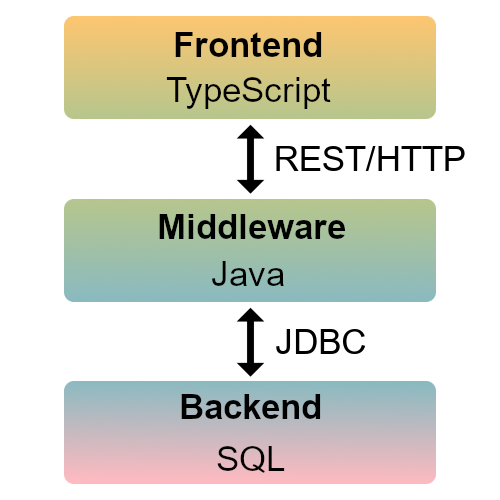
\includegraphics[width=.3\textwidth]{command-structure.png}
    \caption{3-Schichten-Struktur von \textit{FNT Command}}
\end{figure}

\begin{itemize}
    \item \textit{\textbf{Frontend.}} In \textit{TypeScript}, einem Superset\footnote{Als Superset basiert \textit{TypeScript} auf \textit{JavaScript} und wird vollständig zu validem \textit{JavaScript}-Code kompiliert. \cite{ts:2021}} von \textit{JavaScript}, geschrieben, bildet das Frontend die Benutzeroberfläche im Browser ab. Benutzer der Software kommen nur mit dieser Schicht der Software in Berührung.
    \item \textit{\textbf{Middleware.}} Die Middleware von \textit{FNT Command} wird in \textit{Java} programmiert. Die Programmlogik der Software wird in dieser Schicht abgebildet und es findet eine ständige Kommunikation mit beiden umliegenden Schichten statt.
    \item \textit{\textbf{Backend.}} Das Backend dient zur dauerhaften Datenspeicherung und wird durch eine \textit{Oracle}-Datenbank dargestellt. Mithilfe des Java-Frameworks \textit{JDBC} können durch \textit{\ac{SQL}}-Abfragen Daten direkt aus der Middleware angefordert und bearbeitet werden.
\end{itemize}

\newpage
Nicht nur über das Frontend kann von außen mit \textit{Command} kommuniziert werden. Die Software bietet mit der \ac{BGW}-\ac{API} eine abstrahierte und versionsunabhängige Schnittstelle zur Interaktion mit externen Systemen. Konkret wird dabei mit einer \ac{BGE} interagiert, einer abstrakten Repräsentation einer Datenbanktabelle in \textit{Command}. Die \ac{BGW}-\ac{API} setzt sich aus vielen verschiedenen dieser \ac{BGE}s zusammen und folgt hierbei als \textit{RESTful}-\ac{API} den Architekturvorgaben des \ac{REST}. Jeder über die \ac{API} zugänglichen Ressource ist eine eindeutige \ac{URI} zugeordnet, welche eine Identifikation der Ressource im Web erlaubt. \cite{berners:2005} Gemäß \ac{REST} wird zum Informationsaustausch vor allem \ac{HTTP} verwendet. An die verschiedenen \ac{URI}s werden \ac{HTTP}-Anfragen gesendet, um auf die gewünschten Ressourcen zugreifen zu können. \cite{kalin:2013} Die Anfrage liefert eine simple Antwort im \ac{JSON}-Format zurück, ein schlankes Format zum Abbilden von Datenstrukturen, welches für Menschen leicht lesbar ist. \cite[S. 266.]{richardson:2008} 

Die \textit{Command} \ac{BGW}-\ac{API} umfasst fast alle auch über das Frontend zugänglichen Funktionen und bietet so vielfältige Möglichkeiten, die Software direkt über \ac{REST}-Anfragen zu bedienen. Dies ist gerade zum automatisierten Testen von \textit{Command} ein großer Vorteil.


\section{Das Command Integration Framework}\label{sec:cif}
Zwar wird von \textit{Command} nach außen hin als eine große Software gesprochen, jedoch besteht diese aus vielen einzelnen und optionalen Custom-Modulen, welche einige Standardmodule um zahlreiche Funktionalitäten erweitern und vom Kunden nur auf Wunsch zu diesem hinzugefügt werden. So können sich mehrere Instanzen von \textit{Command} bei verschiedenen Kunden deutlich unterscheiden. Eines der erwähnten Custom-Module, welches allerdings seit \textit{Command 13.4} als Standardmodul in \textit{Command} integriert ist, ist das \acf{CIF}.

Unternehmen speichern in der Realität oft große Mengen an Daten dezentral in diversen Softwareprodukten unterschiedlicher Hersteller, was eine Übersicht über diese erschwert und somit ein erhöhtes Risiko für fehlerhaft dokumentierte Daten darstellt. Das \ac{CIF} bietet Nutzern von \textit{Command} die Möglichkeit, Daten aus Fremdsystemen in \textit{Command} zu integrieren und so zentral zu verwalten. Dessen Aufbau ist in der folgenden Abbildung ersichtlich.

\begin{figure}[h]
    \centering
    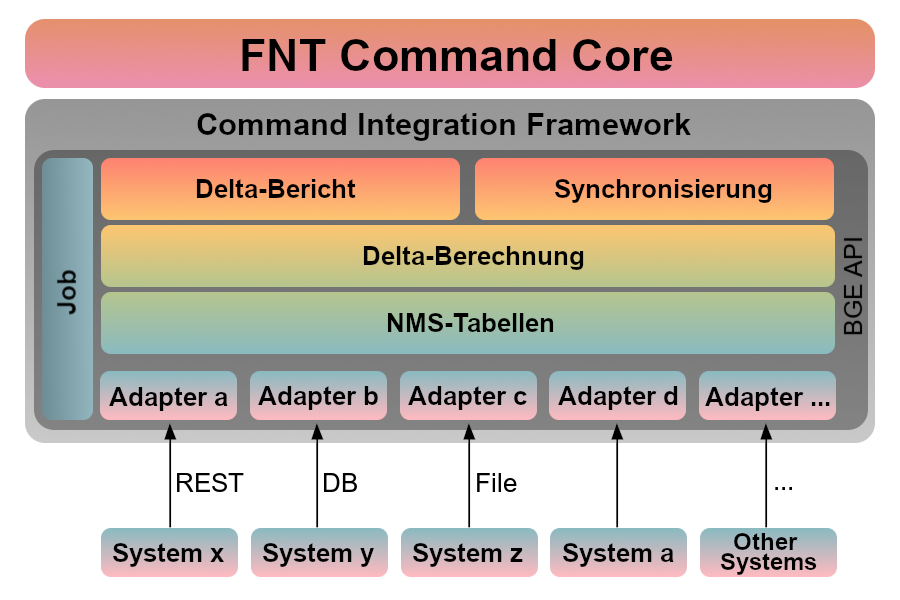
\includegraphics[width=.8\textwidth]{cif-struktur.png}
    \caption{Aufbau des \ac{CIF}}
\end{figure}

Das Fundament für die Datenintegration bilden die sogenannten Adapter. Ein Adapter wird genau passend für ein bestimmtes Fremdsystem eines Kunden entwickelt und dient als Schnittstelle zwischen Fremdsystem und \textit{Command}. Als solche ist der Adapter für den sogenannten \textit{ETL}-Prozess verantwortlich. Dies bedeutet, der Adapter führt eine \textbf{E}xtrahierung der Fremddaten durch, woraufhin die \textbf{T}ransformation der Daten in ein von \textit{Command} erkanntes Format erfolgt und somit ein \textbf{L}aden der transformierten Daten in die \textit{Command}-Datenbank durchgeführt kann.

Die nächste Schicht des \ac{CIF} wird durch sogenannte \textit{Staging-Tabellen}, in \textit{Command} \ac{NMS}-Tabellen genannt, abgebildet. Diese dienen zur Zwischenspeicherung von Daten, nachdem diese von einem Adapter geladen wurden. Daten aus einem Fremdsystem werden nicht sofort in \textit{Command} geladen, sondern zuerst im Staging-Bereich, also in den \ac{NMS}-Tabellen, zwischengespeichert, um eventuell auftretende Diskrepanzen zwischen den in \textit{Command} bereits vorhandenen und den neu geladenen Daten zu erkennen und aufzulösen. Diese Diskrepanzen werden in der Umgebung des \ac{CIF} \textit{Deltas} genannt.

Das Identifizieren dieser Deltas erfolgt im nächsten Schritt durch die sogenannte Delta-Berechnung. Hier wird ein genauer Vergleich der Ist-Daten in der Produktivumgebung mit den vom Fremdsystem importierten Soll-Daten im Staging-Bereich durchgeführt. Anhand der gefundenen Differenzen, der Deltas, wird bestimmt, welche Aktionen für die von den Soll-Daten abweichenden Ist-Daten im späteren Verlauf des Datenintegrationsprozesses durchgeführt werden können, um die Diskrepanzen zu beseitigen und die Ist-Daten auf den Soll-Zustand zu bringen. Diese Aktionen werden \textit{Deltafälle} genannt und werden im Kapitel \ref{sec:deltacases} weiter erläutert.

Für den auf die Delta-Berechnung folgenden Schritt, die Synchronisation der Daten, können Nutzer*innen im Web-Frontend genehmigen, welche Ist-Daten auch tatsächlich zur Auflösung der Deltas verändert werden sollen. Hierfür existiert eine Deltatabelle im \ac{CIF}-Modul in \textit{Command}, welche das manuelle Verwalten von sämtlichen berechneten Deltas erlaubt. Genehmigte Daten werden daraufhin je nach von der Deltaberechnung bestimmter Aktion, also je nach Deltafall, in \textit{Command} an die Daten in der \ac{NMS}-Tabelle im Staging-Bereich angepasst.
 
Die beschriebe Deltaberechnung und Synchronisation kann über einen sogenannten \textit{Job} automatisiert und gesteuert werden. Ein Job kann über das \textit{Command}-Frontend mit verschiedenen Parametern konfiguriert werden und so bei Starten des Jobs automatisch gewünschte Vorgänge nacheinander initiieren. So kann ein Job beispielsweise konfiguriert werden, Deltas einer spezifischen Entitätskategorie wie Devices oder Zonen zu berechnen, diese über eine sogenannte \textit{Delta Auto-Apply-Konfiguration} direkt zu genehmigen und daraufhin zu synchronisieren. So sind vom Start der Delta-Berechnung bis hin zum vollständigen Synchronisieren der Daten keine manuellen Eingriffe nötig.

\section{Deltafälle im CIF}\label{sec:deltacases}
Wie im vorherigen Kapitel angeführt, bezeichnen Deltafälle bestimmte Aktionen, welche für Ist-Daten in \textit{Command}, im Folgenden auch \textit{Command}-Objekte genannt, ausgeführt werden können, um Deltas aufzulösen. So können die \textit{Command}-Objekte an den aktuellen Soll-Zustand der Daten in den \ac{NMS}-Tabellen im Staging-Bereich, im weiteren Verlauf auch \ac{NMS}-Objekte genannt, angeglichen werden.

Bevor die verschiedenen Deltafälle genauer erläutert werden können, bedarf es einer Erklärung, wie genau das \ac{CIF} beziehungsweise \textit{Command} überhaupt Deltas zwischen \ac{NMS}- und \textit{Command}-Objekten erkennen kann. Jedes Objekt in \textit{Command} besitzt mehrere verschiedene Identifikationsmöglichkeiten. Die \ac{Elid} eines Objekts ist ein einzigartiger 14-stelliger alphanumerischer Wert, der bei Erstellung eines Objekts in \textit{Command} automatisch generiert wird und zur eindeutigen Identifikation dient. Ähnlich zur \ac{Elid} ist auch die sogenannte \textit{objectId} einzigartig, jedoch kann diese für ein Objekt auch selbst nach Belieben erstellt werden, solange es den Wert nicht schon in \textit{Command} gibt. Die letzte Identifikationsmöglichkeit ist die \textit{visibleId}. Diese entspricht quasi einer Art Namen eines Objekts und muss im gesamten \textit{Command}-Umfeld nicht einzigartig sein. Tatsächlich wird sich gerade dies für die Delta-Berechnung zu Nutze gemacht. Objekte in \textit{Command} und Objekte in den \ac{NMS}-Tabellen werden über ihre \textit{visibleId}-Werte einander zugeordnet - hierbei nennt sich das Attribut im \ac{NMS}-Bereich lediglich anders, worauf jedoch in den Kapiteln \ref{ch:sollzustand} und \ref{ch:realisierung} näher eingegangen wird. Für das Verständnis ist an diesem Punkt nur relevant, dass ein Ist- und ein Soll-Objekt über korrespondierende ID-Attribute als zusammengehörig erkannt werden. Existiert also ein \textit{Command}-Objekt mit \textit{visibleId} \enquote{TEST\_CHASSIS\_1} und ein \ac{NMS}-Objekt mit demselben Wert für das entsprechende Attribut, so erkennt \textit{Command} das \textit{Command}-Objekt als Ist- und das \ac{NMS}-Objekt als Soll-Zustand für ein aus der Realität abgebildetes Objekt und kann so Deltas und zugehörige Deltafälle berechnen.

Die für diese Arbeit relevanten Deltafälle sollen in der folgenden Liste jeweils kurz erläutert werden.
\begin{itemize}
    \item \textbf{CREATE:} Ein Objekt ist in der \ac{NMS}-Tabelle vorhanden, nicht aber in \textit{Command}. Es soll also in \textit{Command} kreiert werden.
    \item \textbf{DELETE:} Ein Objekt ist nicht in der \ac{NMS}-Tabelle vorhanden, dafür aber in \textit{Command}. Es soll also aus \textit{Command} gelöscht werden.
    \item \textbf{UPDATE:} Ein Objekt ist in der \ac{NMS}-Tabelle vorhanden und in \textit{Command}, jedoch unterscheiden sich Attributwerte zwischen beiden Objekten. Es soll also das Objekt in \textit{Command} mit den neuen Werten vom \ac{NMS}-Objekt aktualisiert werden.
    \item \textbf{UPDATE\_TYPE:} Dieser Deltafall ist dem Fall \enquote{UPDATE} sehr ähnlich. Ein Objekt ist in der \ac{NMS}-Tabelle vorhanden und in \textit{Command}, jedoch unterscheidet sich ein bestimmter Attributwerte zwischen beiden Objekten - der Typ. Es soll also das Objekt in \textit{Command} mit dem neuen Typ beziehungsweise Device Master vom \ac{NMS}-Objekt aktualisiert werden.
\end{itemize}

Diese vier Deltafälle werden auch als reale Deltafälle bezeichnet, da sie Objekte in Echtzeit betreffen. Zusätzlich gibt es in \textit{Command} es die Möglichkeit, Objekte für eine künftige Erstellung oder Löschung zu planen. Die Objekte werden hierbei mit einer speziellen Markierung in \textit{Command} platziert, die aussagt, ob die Objekte in Zukunft in einen realen Zustand übergehen sollen oder on geplant ist, diese aus \textit{Command} zu entfernen. 

\begin{itemize}
    \item \textbf{PLANNED\_CREATE:} Ein Objekt ist in \textit{Command} als zur Erstellung geplant markiert und auch in der \ac{NMS}-Tabelle vorhanden. Bei der Synchronisation wird das Objekt aus dem Planungsstatus gelöst und als reales Objekt in \textit{Command} erstellt.
    \item \textbf{PLANNED\_DELETE:} Ein Objekt ist in \textit{Command} als zur Löschung geplant markiert und nicht in der \ac{NMS}-Tabelle vorhanden. Bei der Synchronisation wird das Objekt aus dem Planungsstatus gelöst und aus \textit{Command} gelöscht.
    \item \textbf{PLANNED\_CREATE\_BUT\_WITH\_DIFFERENT\_TYPE:} Ein Objekt ist in \textit{Command} als zur Erstellung geplant markiert und auch in der \ac{NMS}-Tabelle vorhanden, jedoch besitzt es dort einen anderen Typ. Bei der Synchronisation wird das Objekt aus dem Planungsstatus gelöst und als reales Objekt mit dem neuen Typen vom \ac{NMS}-Objekt in \textit{Command} erstellt.
    \item \textbf{PLANNED\_DELETE\_WITH\_CREATE:} Ein Objekt ist in \textit{Command} als zur Löschung geplant markiert und zwar in der \ac{NMS}-Tabelle vorhanden, jedoch besitzt es dort einen anderen Typ. Bei der Synchronisation wird das \textit{Command}-Objekt aus dem Planungsstatus gelöst und zunächst gelöscht. Ein komplett neues \textit{Command}-Objekt wird daraufhin als reales Objekt mit dem neuen Typen vom \ac{NMS}-Objekt in \textit{Command} erstellt.
    \item \textbf{PLANNED\_DELETE\_WITH\_PLANNED\_CREATE\_BUT\_WITH\_\newline DIFFERENT\_TYPE:} Ein Objekt ist in \textit{Command} als zur Löschung geplant markiert und ein weiteres \textit{Command}-Objekt mit derselben \textit{visibleId}, jedoch einem anderen Typen, ist als zur Erstellung geplant markiert. In der \ac{NMS}-Tabelle befindet sich ein Objekt mit einem Typen, welcher sich wiederum von dem zur Erstellung markierten Objekt unterscheidet. Bei der Synchronisation wird das erste \textit{Command}-Objekt zunächst gelöscht und daraufhin das zweite mit dem neuen Typen vom \ac{NMS}-Objekt als real in \textit{Command} erstellt.
    \item \textbf{PLANNED\_DELETE\_WITH\_PLANNED\_CREATE:} Ein Objekt ist in \textit{Command} als zur Löschung geplant markiert und ein weiteres \textit{Command}-Objekt mit derselben \textit{visibleId}, jedoch einem anderen Typen, ist als zur Erstellung geplant markiert. In diesem Fall enspricht der Typ des \ac{NMS}-Objekts allerdings dem des zu erstellenden \textit{Command}-Objekts, sodass das erste Objekt gelöscht und das zweite ohne Typänderung real in \textit{Command} erstellt werden kann.
\end{itemize}

Es existieren noch einige weitere Deltafälle, welche für das Verständnis dieser Arbeit allerdings keine wirkliche Relevanz besitzen, sodass auf einer weitere Erläuterung dieser verzichtet wird.

\section{Software Testing}\label{sec:swtesting}
Dieses Unterkapitel beschreibt einige theoretische Grundlagen zum Testen von Software und schafft damit eine Basis zum Verständnis des \ac{CIF}-Testprojekts und der darauf basierenden automatischen Testdatengenerierung.

\subsection{Grundsätze des Software Testing}\label{subsec:testinginqa}
Um effektive Tests für ein System definieren zu können, muss sich ein*e Tester*in einiger Grundsätze bewusst sein. Ohne dieses Bewusstsein ist es nur schwer oder gar nicht möglich, Software ausreichend und für das Unternehmen wirtschaftlich lohnend zu testen. Diese folgenden Grundsätze zum Testen von Software gelten für jede Art von Softwaretest.
\begin{itemize}
    \item Software wird mit der Intention getestet, Fehler zu finden. \cite[S. 6]{myers:2011}\cite[S. 11]{witte:2019}
    \item Die völlige Korrektheit von Software kann nicht gezeigt werden, sondern lediglich, dass sie ihre erwünschte Funktion erfüllt. \cite[S. 19]{ammann:2016}\cite[S. 12]{witte:2019}
    \item Software sollte so früh wie möglich getestet werden. Je früher Fehler in einem System entdeckt werden, desto weniger Aufwand bereitet das Beheben dieser und desto weniger Kosten entstehen für das Unternehmen. \cite[S. 12]{witte:2019} \cite[Fig. 1.3]{desikan:2006}
    \item Wird ein Fehler in einem System gefunden, muss davon ausgegangen werden, dass weitere Fehler auftreten können. Diese treten in der Regel gehäuft in einer einzelnen Softwarekomponente auf und nicht gleichmäßig verteilt auf das ganze System. \cite[S. 13]{witte:2019}
    \item Tests verlieren auf Dauer ihre Wirksamkeit. Sie müssen daher ständig an das sich stetig verändernde \ac{SUT} angepasst werden. \cite[S. 13f.]{witte:2019}
    \item Tests müssen nachvollziehbar sein und dokumentiert werden. \cite[S. 14f.]{witte:2019}
\end{itemize}

Unter diesen Gesichtspunkten wird deutlich, dass Testsuites für jedes \ac{SUT} aktiv geplant und gepflegt werden müssen. Es muss genau definiert werden, welche Testfälle möglich sind und welche davon umgesetzt werden können, um die Kosten für die Testimplementierung und -durchführung möglichst gering zu halten und dabei gleichzeitig für eine bestmögliche Testabdeckung zu sorgen.

\subsection{Verschiedene Konzepte zum Testen von Software}\label{subsec:testkonzepte}
In Anbetracht der Vielfalt von Software und deren Architektur ist es nicht möglich, mit einer einzigen strikten Herangehensweise an das Testen von Software jedwedes zu testende Stück Code abzudecken. Daher sind für diverse Situationen unterschiedliche Testkonzepte und -methoden entstanden. Für einige davon soll im Folgenden eine Übersicht gegeben werden.

\subsubsection*{Whitebox Tests}\label{subsubsec:whitebox}
Werden auch als strukturelle Tests bezeichnet, da hierbei die interne Struktur des \ac{SUT} als Testbasis dient. Dies bedeutet, dass das System beim Testen völlig transparent und der Programmcode für die zu testende Programmfunktionalität einsehbar ist und so bestimmte Codezweige gezielt getestet werden können. \cite[S. 125f.]{oregan:2019} Whitebox Tests sind hierbei als Überbegriff für sämtliche Testverfahren anzusehen, welche ihre Tests direkt auf dem Code basieren. Dazu zählen beispielsweise Unittests, welche im weiteren Verlauf separat erläutert werden sollen. 

\subsubsection*{Blackbox Tests}\label{subsubsec:blackbox}
Ähnlich wie das Whitebox Testing ist auch das Blackbox Testing lediglich ein Überbegriff für diverse Arten von Tests. Wie sich schon am Namen ableiten lässt, stellen Blackbox Tests dabei das Gegenteil zu den Whitebox Tests dar. Sie werden auch als spezifikationsorientierte Tests bezeichnet, da sie lediglich auf das Verifizieren der korrekten Funktionalität, also den geforderten Spezifikationen, eines Systems ausgerichtet sind. Das System selbst bleibt dabei eine sogenannte Blackbox, was bedeutet, dass die innere Struktur des \ac{SUT} unbekannt ist. \cite[S. 120f.]{oregan:2019}

\subsubsection*{Greybox Tests}\label{subsubsec:greybox}
Greybox Tests stellen eine Mischform zwischen Blackbox und Whitebox Tests dar. Der Test wird wie beim Whitebox-Unittest (s. unten) vom Entwickler speziell für seinen Code geschrieben, allerdings bevor der Code selbst implementiert wird, womit die noch nicht bekannten genauen Details des zu testenden Codes den Blackbox-Aspekt wiederspiegeln. \cite[S. 86]{witte:2019}

\subsubsection*{Unittests}\label{subsubsec:unittest}
Unittests werden auch als Modultests bezeichnet und sind ein Whitebox-Testverfahren. In der Regel werden Unittests direkt von Entwicklern passend für den von ihnen neu implementierten Code geschrieben. Funktionale Einzelteile der Software, Module, werden dabei auf korrekte Funktionalität geprüft. \cite[S. 75]{witte:2019}

\subsubsection*{Integrationstests} \label{subsubsec:integrationstests}
Integrationstests dienen der Prüfung des Zusammenspiels verschiedener Komponenten von Software miteinander. Hierfür wird eine Reihe von Tests aufeinander abgestimmt. Es können so beispielsweise fehlerhafte Schnittstellen oder falsche Dateninterpretationen zwischen Komponenten aufgedeckt werden. \cite[S. 76]{witte:2019}

\subsubsection*{Systemtests}\label{subsubsec:e2etests}
Werden auch als \ac{E2E}-Tests bezeichnet. Mit diesen Tests wird das gesamte \ac{SUT} auf bestimmte funktionale und nicht funktionale Anforderungen getestet. Hierfür werden die Tests auf einer möglichst produktionsähnlichen Testumgebung ausgeführt. \cite[S. 78f.]{witte:2019} Diese Tests stellen die Mehrheit der Tests in Projekt \enquote{CIF Automated Tests} dar.

\subsubsection*{GUI-Tests}\label{subsubsec:guitests}
Die korrekte Funktionalität und die Benutzerfreundlichkeit der \ac{GUI} beziehungsweise der Web-Oberfläche wird getestet. Funktionalitäten, die im Backend funktionieren, müssen auch bei Ausführung über die \ac{GUI} funktionieren. \cite{bruns:2009} \ac{GUI}-Tests sind allerdings langsam und werden daher meist in geringerer Anzahl umgesetzt. \cite{contan:2018}

\subsubsection*{Manuelles Testen}\label{subsubsec:manuelltest}
Alle Arten von Tests können manuell oder automatisiert ausgeführt werden. Manuelles Testen bedeutet, dass ein*e Tester*in händisch alle zum Ausführen einer Funktionalität erforderlichen Schritte ausführt und das Ergebnis mit einem zu erwartenden Ergebnis vergleicht. Dieser Prozess kann dabei sehr aufwendig werden und mehrere Wochen dauern (s. Anhang \nameref{app:befragung}, Frage 4). Jedoch können durch manuelles Testen viele Fehler gerade in neuen Funktionalitäten aufgedeckt werden, welche noch nicht Teil der automatisierten Testsuite sind \cite[S. 231]{witte:2019} (s. Anhang \nameref{app:befragung}, Frage 7).

\subsubsection*{Automatisiertes Testen}\label{subsubsec:autotest}
Insbesondere der Zeitfaktor beim manuellen Testen macht die Testautomatisierung für Unternehmen attraktiv. Wiederholt ausgeführte Tests werden durch ein Skript automatisiert ausgeführt, sodass bis zu 80\% des Testaufwands im Vergleich zu manuellem Testen gespart werden kann. \cite[S. 3]{fewster:1999} Diese Zeit können manuelle Tester*innen wiederum zum Testen neuer Releases und Funktionalitäten verwenden, worin sie automatisierten Testskripten überlegen sind. \cite[S. 231]{witte:2019} Trotz der auf lange Sicht lohenswerten Zeitersparnis und Effizienzsteigerung sind auch automatisierte Tests zumindest in der Implementierung und Wartung sehr ressourcenaufwendig. \cite[S. 5]{fewster:1999}

Automatisiertes Testen harmoniert mit dem Prinzip der agilen Softwareentwicklung, da bei jeder Softwareiteration die bestehenden Tests effizient automatisch ausgeführt und mit der neuesten Iteration ins System eingeführte Fehler aufgedeckt werden können. \cite{contan:2018} \cite{fewster:1999} Automatisierte Tests werden hierbei zumeist gemäß der Pyramide zur Testautomatisierung, welche von Mike Cohn erstmals 2009 definiert wurde, strukturiert. \cite{cohn:2010} Diese Pryamide ist im Folgenden abgebildet.

\begin{figure}[h]
    \centering
    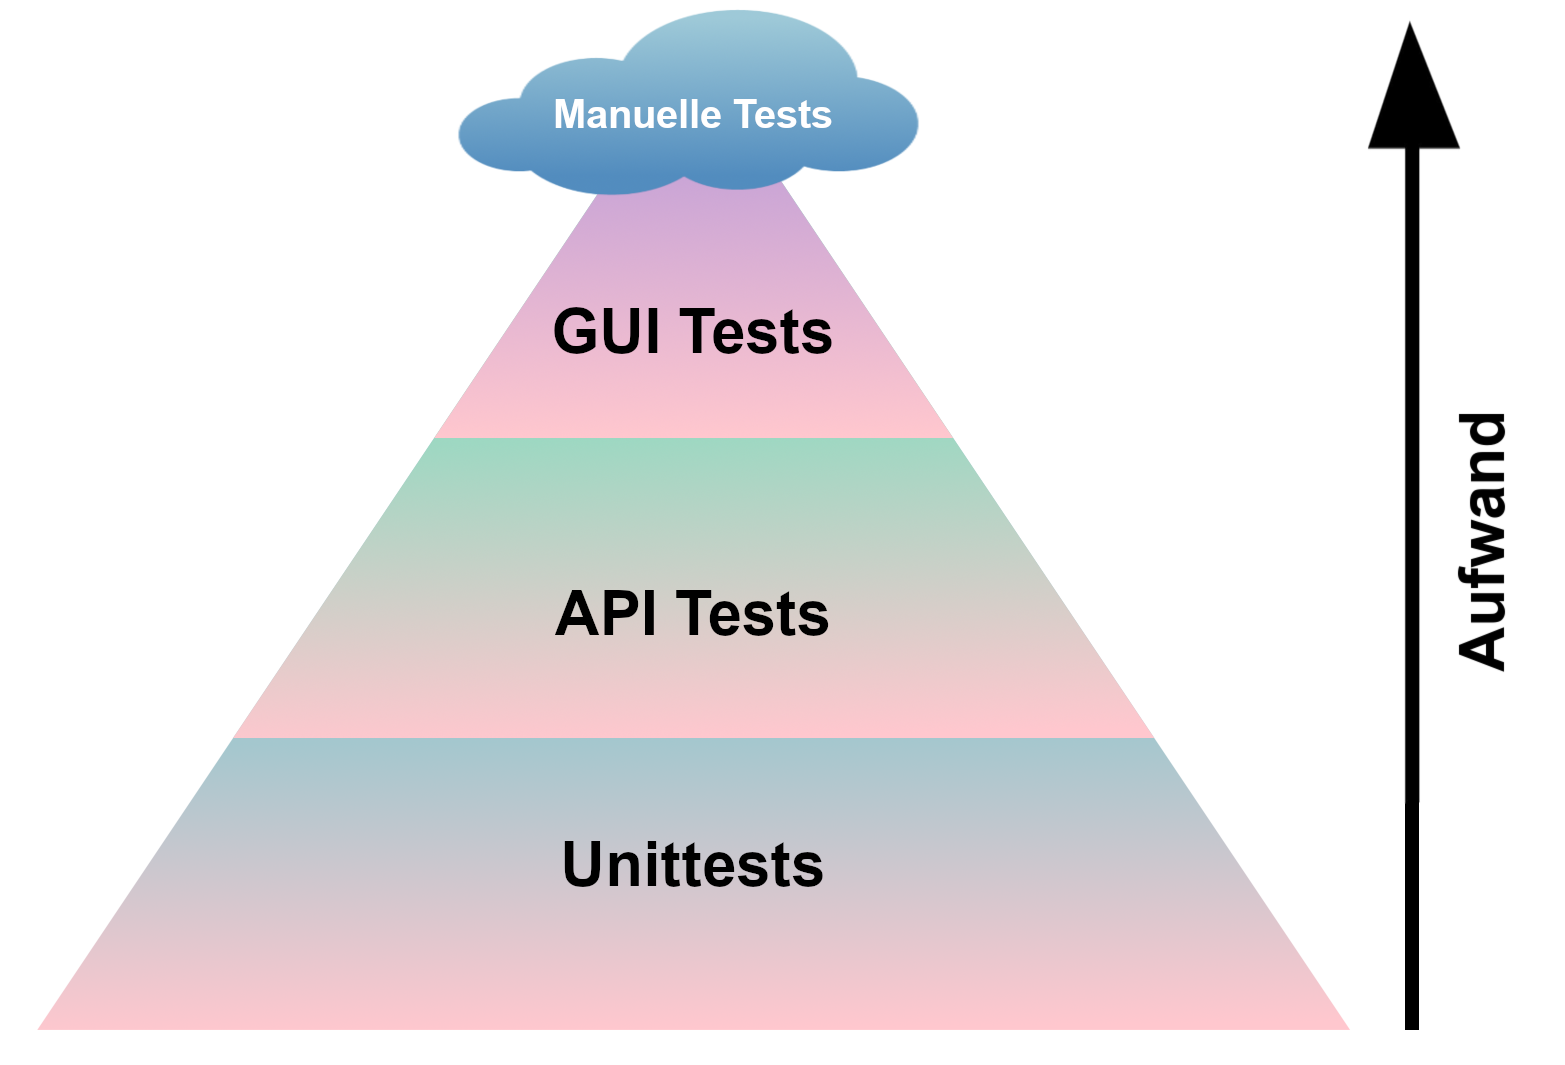
\includegraphics[width=.7\textwidth]{testing-pyramid.png}
    \caption{Pyramide zur Testautomatisierung}
\end{figure}

Nach der Testautomatisierungspyramide werden die meisten automatisierten Tests als Unittests realisiert, da diese mit dem geringsten Aufwand verbunden sind. Darauf folgen \ac{API}-Tests wie Integrationstests und \ac{E2E}-Tests. Als \ac{GUI}-Tests werden aufgrund des größeren Testaufwands die wenigsten Tests realisiert. Trotz automatisierter Tests bleiben aber immer Testfälle, welche nur durch manuelles Testen abgedeckt werden können - dies wird durch die Wolke an der Spitze der Pyramide dargestellt.

\subsection{Die Bedeutung von Testdaten für effektives Software Testing}\label{subsec:testdaten}
Die Qualität von Softwaretests wird durch vielerlei Faktoren beeinflusst. Ein Faktor, der hierbei bisweilen als fast selbstverständlich angesehen wird, ist das Vorhandensein von Testdaten. Diese können entscheidend dafür sein, ob ein Test, sei er noch so korrekt implementiert und ausgeführt, überhaupt brauchbare Ergebnisse liefern kann.

Testdaten von schlecher Qualität können der Grund sein, weshalb Tests nicht das erwartete Ergebnis anzeigen. \cite[S. 137]{oregan:2019} Ein konkretes Beispiel hierfür in der \ac{CIF}-Testumgebung kann in der Deltaberechnung theorisiert werden. Wenn der Deltafall \enquote{UPDATE} getestet werden soll, erwartet \textit{Command}, dass sich zwei Objekte mit derselben \textit{visibleId} in der \ac{NMS}-Tabelle und in \textit{Command} befinden, sich aber in bestimmten Attributwerten unterscheiden. Kam es nun aber beispielsweise bei der Erstellung der Daten zu einem Tippfehler in der \textit{visibleId}, sodass die beiden Objekte sich hierin nicht mehr entsprechen, erkennt \textit{Command} den Deltafall nicht als \enquote{UPDATE}, sondern für das \ac{NMS}-Objekt als \enquote{CREATE} und für das Objekt in \textit{Command} als \enquote{DELETE}. Der Deltafall \enquote{UPDATE} wird also gar nicht getestet; in diesem Fall würde aber der Test zumindest fehlschlagen und dadurch vermitteln, dass etwas nicht stimmt. Testdaten bestimmen also direkt den Verlauf des Testfalls, denn nur mit bestimmten Werten der Testdaten wird auch der gewünschte Pfad im \ac{SUT} eingeschlagen. \cite[S. 221]{witte:2019}

Um das Beispiel weiterzuführen, wird nun angenommen, in \textit{Command} existiere ein Bug bei der Erkennung des Deltafalls \enquote{UPDATE}. Mit korrekten Testdaten könnte dieser Bug leicht identifiziert werden. Wenn aber die Testdaten schon zu verfälschten Ergebnissen führen, könnte es im schlimmsten Fall dazu kommen, dass durch den Bug in der Software der eigentlich falsch berechnete Deltafall als korrekt angesehen wird. Der Test verschleiert in diesem Fall also den Bug in der Software - aufgrund eines einfachen Fehlers wie eines Tippfehlers in der \textit{visibleId}.

Auch Testdaten von hoher Qualität können mit der Zeit ihre Gültigkeit verlieren, wenn Testfälle oder die Testumgebung verändert werden. Testdaten müssen daher immer wieder geprüft und gegebenenfalls angepasst werden. \cite[S. 121f.]{witte:2019} Die Erstellung und Pflege von validen Testdaten nimmt also auch beträchtliche Zeit und Ressourcen in Anspruch, wie auch von Tester*innen bei \textit{FNT} bestätigt wurde. Fast jede Woche müssen Anpassungen an Testdaten vorgenommen werden, weil diese durch unbeabsichtigte Änderungen an den Daten selbst oder Änderungen der Funktionalität des Systems auftreten, die mit den veralteten Testdaten Tests fehlschlagen lassen. (s. Anhang \nameref{app:befragung}, Frage 10)

Testdaten sind auch ein fester Bestandteil in der Festlegung der Teststrategie für ein beliebiges \ac{SUT}. Es muss beschrieben werden, welche Testdaten verwendet werden, wo sie abgelegt sind und wie sie organisiert werden. \cite[S. 119]{witte:2019} Insbesondere in der Testautomatisierung kommt einer konsequenten Testdatenverwaltung ein besonderer Stellenwert zu, denn automatisierte Tests erfordern eine gegebene Konfiguration der Testdaten zu Beginn der Testaktivitäten. \cite[S. 236]{witte:2019}

Glenford J. Myers sagt Folgendes über Testinputs:

\enquote{\textit{In general, the least effective methodology of all is random-input
testing — the process of testing a program by selecting, at random, some
subset of all possible input values. In terms of the likelihood of detecting
the most errors, a randomly selected collection of test cases has little
chance of being an optimal, or even close to optimal, subset.}} \cite[S. 41]{myers:2011}

Mit zufällige Inputdaten als schlechtester Möglichkeit zum effektiven Testen von Software folgt daraus im Umkehrschluss, dass Testdaten so real und exakt wie möglich auf den Use-Case zugeschnitten sein müssen, um effektiv testen zu können. Auch dies wird von befragten Tester*innen bei \textit{FNT} bestätigt. (s. Anhang \nameref{app:befragung}, Frage 8)

Unter Berücksichtigung dieser Gesichtspunkte lässt sich schlussfolgern, dass Testdaten einen hohen Stellenwert für die Qualität der Softwaretests allgemein besitzen, da sie die Basis für Softwaretests darstellen. Ohne qualitativ hochwertige Testdaten können die Tests gar nicht erst ausgeführt werden oder deren Ergebnisse werden verfälscht und damit unbrauchbar. Im schlimmsten Fall kann ein mit unpassenden Testdaten asugeführter Test sogar ein falsches Positiv erzeugen, was eine nicht gegebene Sicherheit vermittelt und einen eventuellen Fehler verschleiert. Besteht also eine Möglichkeit, für ein Unternehmen den Testdatenerstellungsprozesses zuverlässiger zu gestalten, sollte dies in jedem Fall genauer analysiert werden.

\subsection{Testdatengenerierungsprinzipien}\label{subsec:grundlagenDatengenerierung}
Die automatische Testdatengenerierung bietet einen interessanten Ansatz, die Qualität von Testdaten gerade im automatisierten Testprozess zu verbessern. 

Nach eigener Definition ist ein Testdatengenerator ein Programm, welches durch bestimmten Input einen Ansatz für die Konstruierung synthetischer Daten bekommt und daraufhin diese Daten in einem bestimmten Format passend für später auszuführende Softwaretests zurückliefert.

Solche Generatoren können entweder komplett selbst implementiert oder auf ein bereits vorhandenes Tool von Drittanbietern zurückgegriffen werden, welches die Datengenerierung entweder komplett übernimmt oder beispielsweise mithilfe von Bibliotheksmethoden zumindest Teilschritte davon unterstützen kann. Solche Tools werden im Kapitel \ref{sec:toolanalyse} ausführlich analysiert.

Das Ziel der automatischen Testdatengenerierung ist das komplett automatisierte Erstellen von synthetischen Testdaten, die eine Produktivumgebung möglichst genau simulieren. Im Optimalfall werden diese Daten dann in jedem Testzyklus valide generiert und so Syntax- oder Semantikfehler, welche durch manuelles Pflegen von Daten eingeführt werden können, vermieden. Diese zu generierenden Testdaten können beliebige Formate annehmen. Es können synthetische Daten speziell so generiert werden, dass sie direkt in \ac{SQL}-Datenbanken eingefügt werden können. Wieder andere Anwendungsfälle können das Erstellen von Test-Dateien in Formaten wie \ac{XML}, \ac{CSV} oder \ac{JSON} sein. Schließlich besteht auch die Möglichkeit, Testdaten gar nicht direkt in dedizierten Speicherorten wie Datenbanken oder Dateien abzulegen, sondern diese nur im Programm selbst, also quasi \enquote{In-Memory}, zu halten und direkt weiterzuverwenden.

Das Generieren dieser synthetischen Daten verläuft über das Analysieren und Imitieren realer Daten. Es werden einem Datengenerator beispielsweise reale Daten gegeben, welche von diesem verändert werden - dies ist häufig aufgrund des Datenschutzes nötig. Weiterhin kann aus einer ausführlichen Analyse der inneren Struktur des \ac{SUT} auf die benötigte Struktur von Testdaten geschlossen werden. Eine weitere Möglichkeit besteht darin, einen Testdatengenerator mit einer oder mehreren vordefinierten Konfigurationen zu versorgen, welche die Struktur oder bestimmte Anforderungen an die erwarteten Testdaten dokumentieren. Eine solche Struktur kann beispielsweise durch die nötigen Attribute und Datentypen der Attribute eines Testdatenobjekts dargestellt werden. Anforderungen können sein, wie viele Testdaten generiert und für welche Use-Cases diese generiert werden sollen. Auf diese verschiedenen Methodiken wird in Kapitel \ref{subsec:methodiken} noch näher eingegangen.

\begin{figure}[h]
    \centering
    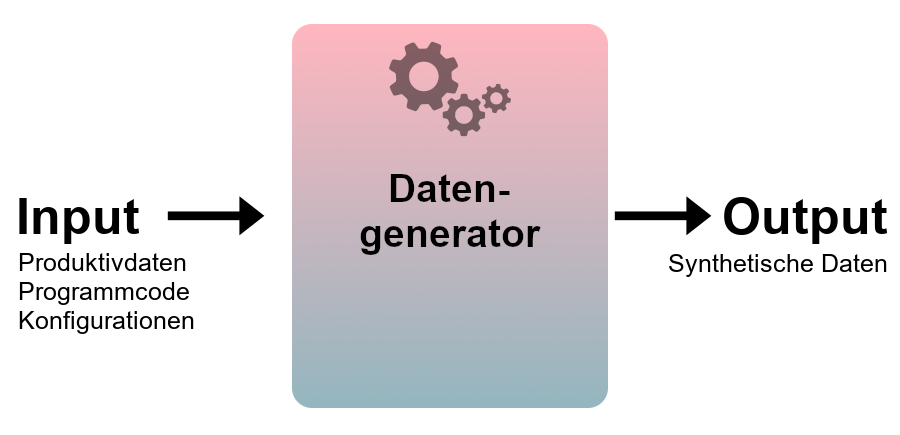
\includegraphics[width=.8\textwidth]{datengenerator.png}
    \caption{Sinngemäßer Ablauf einer Datengenerierung}
\end{figure}